%\chapter{納豆菌の菌糸直径計測および菌糸本数推定手法}
%\section{納豆菌の直径計測手法}
%\section{納豆菌の菌糸本数推定手法}

\chapter{提案システム}

提案システムでは,教室などの閉鎖空間において,
個人が所有する複数のスマートデバイスの音声出力をネットワークを介し同期させ制御することで,スピーカアレイを構築する(図\ref{fig:shikumi2}).
空間内に配置した仮想音源の位置に基づき,その音源位置を囲む最寄りの3つのスマートデバイス(ノード)を設定し振幅パニングすることで,現実世界における想定位置で音源を鳴らして定位する.
このようなスピーカアレイを構築するにあたり,実空間に分布する複数のスマートデバイスの相対位置を推定するとともに,端末間での時刻同期が必要不可欠である.

\begin{figure}[p]\centering
  \hspace{-2mm}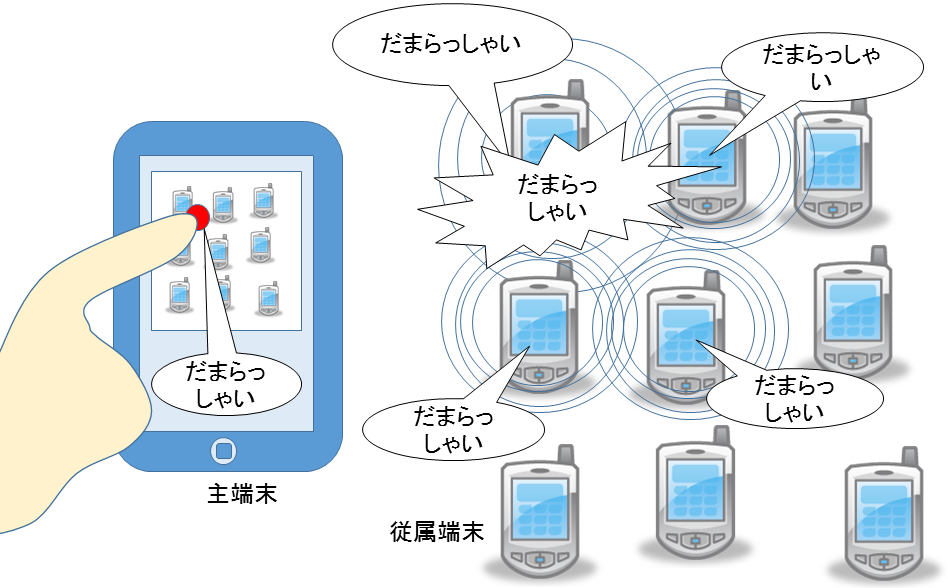
\includegraphics[clip,width=1.1\hsize]{img/shikumi3.png}
  \caption{提案システムの概念}\label{fig:shikumi2}
\end{figure}

この章では,まず,提案システムで用いた
相対位置に基づく音像定位手法について触れる.
次に,その手法を実現するための
端末間の音声パルスの到達時間差による
時刻同期手法および相対距離計測手法,
そして相対位置推定手法を述べる.
さらに,パルス圧縮を用いた信号検出手法を示し,
最後に,スピーカアレイ全体の制御手法について解説する.



\section{DBAP法を用いた音像定位}

はじめに,複数のスマートデバイスを使ってどのように音像定位するのかについて述べる.
今回のような平面配置のスピーカアレイを用いて音像定位をする手法として,
Distance-based amplitude panning (DBAP) 法\cite{dbap}がある.

DBAP法は,
任意の数のスピーカの位置が既知であり,
端末間のスピーカの出力特性が等しいとしたときに,
仮想音源と各スピーカとの距離から距離減衰を計算することで,
各スピーカの振幅を制御して音像を合成する手法である.

位置 $(x_s,y_s)$ にある仮想音源 $VS$ から,
位置 $(x_i,y_i)$ にある端末 $i$ への距離 $d_i$ を次のように定義する(図\ref{fig:DBAP}).

\begin{figure}[p]\centering
  \hspace{-2mm}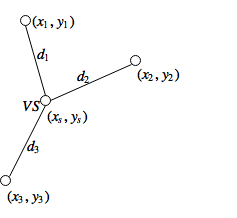
\includegraphics[clip,width=1.1\hsize]{img/DBAP.png}
  \caption{DBAP}\label{fig:DBAP}
\end{figure}

$$
d_i = \sqrt{(x_i - x_s)^2 + (y_i - y_s)^2} \qquad (\mathrm{for}\ 1 \leq i \leq N)
$$

DBAP法では,仮想想源の位置に関係なく,各スピーカからの音の強さの合計は

$$
I = \sum_{i=1}^N v_i^2 = 1
$$

として正規化している.
$i$ 番目のスピーカの相対的な振幅は距離に反比例するので

$$
v_i = \frac{k}{d_i^a}
$$

と定義できる.
$k$ はすべてのスピーカと仮想音源の位置に依存した係数で,

$$
k = \frac{1}{\sqrt{\sum_{i=1}^N \frac{1}{d_i^{2a}}}}
$$

である.
係数 $a$ は距離減衰係数で

$$
a = \frac{R}{20 \log_{10}2} \\
$$

と定義する.
$R$ はロールオフ係数で,受聴者と音源の距離に基づく減衰の量である.
$R=6\ [\mathrm{dB}]$ の場合は,
自由空間における距離減衰の逆二乗則に基づき,音の強さのレベルが音源からの距離が2倍になるごとに6dBずつ減少することを意味する.
また,半自由空間では $R=3\sim5\ [\mathrm{dB}]$ 程度となる.

以上のとおり,
複数のスマートデバイスが
同期的に制御でき,
端末の位置が判明しており,
端末間のスピーカの出力特性が均一であれば,
この手法を用いて音像定位ができることが分かった.



\section{時刻同期と測距}

基準となる時刻が違う二つの時間軸を持つ端末間において同期するには,
互いに音声パルスを出せばよい(図\ref{fig:beeptobeep}).

\begin{figure}[p]\centering
  \hspace{-2mm}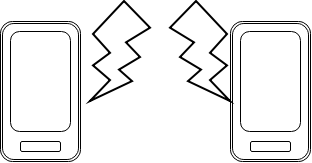
\includegraphics[clip,width=1.1\hsize]{img/beeptobeep.png}
  \caption{beeptobeep}\label{fig:beeptobeep}
\end{figure}

この手法はTPSN(time-sync Protocol for sensor network)\cite{tpsn}
などで提案されている.
原理を説明する.

端末 $A$ が自身の時刻 $t_0$ に音声パルスを発生すると,
そのパルスは音速で空間に広がり,
端末 $B$ 内の時刻 $t_1$ に受信される.
さらに,端末 $B$ からも端末 $B$ 内の時刻 $t_2$ に音声パルスを発すると,
このパルスも音速で空間に広がり,
端末 $A$ 内の時刻 $t_3$ に受信される.
ここで,図の通り,
端末 $A$ 内のパルス時間間隔 $t_3-t_0$ と
端末 $B$ 内のパルス時間間隔 $t_2-t_1$ には差が生じる(図\ref{fig:clocksynchronization}).

\begin{figure}[p]\centering
  \hspace{-2mm}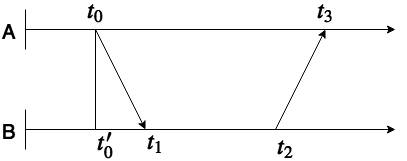
\includegraphics[clip,width=1.1\hsize]{img/clock_synchronization.png}
  \caption{clocksynchronization}\label{fig:clocksynchronization}
\end{figure}

パルスの往復で伝播にかかった時間は共に等しいと仮定すると,

$$
t_0' = t_1 - \frac{(t_3 - t_0) - (t_2 - t_1)}{2} \\
$$

となり,端末 $B$ 内時刻で端末 $A$ のパルスが発せられた時刻を推定することができる.
以上が時刻同期の原理である.

音速を $c$ とすれば,副次的に端末間の距離も求まる.

$$
d_{AB} = \frac{(t_3 - t_0) - (t_2 - t_1)}{2c}
$$

端末AB間で何らかの処理を同期的に実行したい場合は
図のようにして実行すべき時間を求められる(図\ref{fig:flowchart3}).

\begin{figure}[p]\centering
  \hspace{-2mm}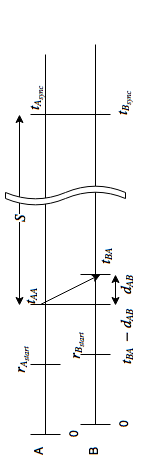
\includegraphics[clip,width=1.1\hsize]{img/flowchart3.png}
  \caption{同期実行}\label{fig:flowchart3}
\end{figure}

基準となる端末Aのパルスの受信時間およびその信号の伝達時間と,
それを受信してからの経過時間 $S$ をもとに,同期的に処理を実行できる.

こうして,端末間の時刻同期と距離測定ができた.



\section{相対位置推定}


次に,複数のスマートデバイスの空間分布をどう推定するかについて述べる.
次のように定式化し誤差関数を最小化する最適化問題を考える.

$$
\varepsilon(\hat{x_1}, \dots, \hat{x_N}) = \sum_{i=1}^N \sum_{j\in M(i)} \left( \| \hat{ x_i } - \hat{ x_j } \| - d_{ij} \right)^2 \\
%\DeclareMathOperator*{\argmin}{arg\,min}
(\hat{x_1} \dots \hat{x_N}) = \mathrm{argmin} \varepsilon(\hat{x_1} \dots \hat{x_N})
$$

ここで,
$N \in \mathbb{N}$ は端末の数,
$M(i) \subset \{1,\dots,N\}$ は端末 $i$ と相対距離が計測できた端末の集合,
$d_{ij} \in \mathbb{R}$ は実際に計測された端末の距離とし,
$\hat{ x_i } \in \mathbb{R}^2$ n番目の端末の位置推定値で,初期値は乱数を置く.

最急降下法を使って反復的に解く.更新式は次のようになる.

$$\begin{aligned}
\hat{x_i} (n + 1) & = \left. \hat{x_i} (n) - a \frac{\partial \varepsilon}{\partial \hat{x_i}} \right|_{\hat{x} = \hat{x}(n)} \\
\frac{\partial \varepsilon}{\partial \hat{x_i}}
&= \sum_{j\in M(i)} \frac{\partial \left( \|\hat{ x_i } - \hat{ x_j }\| - d_{ij} \right)^2}{\partial \hat{x_i}} \notag\\
&= 2 \sum_{j\in M(i)} \left( \| \hat{x_i} - \hat{x_j} \| - d_{ij} \right) \frac{\partial \| \hat{x_i} - \hat{x_j} \|}{\partial \hat{x_i}} \notag\\
&= 2 \sum_{j\in M(i)} \left( 1 - \frac{d_{ij}}{\| \hat{x_i} - \hat{x_j} \|} \right) \left( \hat{x_i} - \hat{x_j} \right).
\end{aligned}$$

$n$ は反復回数, $a$ は更新式のステップ幅である.
図\ref{fig:relpo_s}にすべての端末間で距離が取得できたとしたシミュレーション結果を示す.


\begin{figure}[p]\centering
  \hspace{-2mm}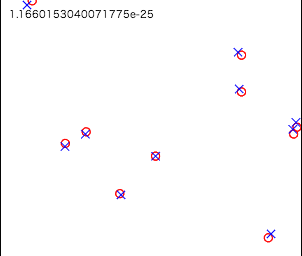
\includegraphics[clip,width=1.1\hsize]{img/positiondetection-new.png}
  \caption{最急降下法によって相対位置を解いたシミュレーション結果}\label{fig:relpo_s}
\end{figure}

端末 $i$ が測距できた他の端末の集合 $M(i)$ は後述する信号検出により決まる.


\section{信号検出}

精密な測距・時刻同期のためには精密な信号検出が必要である.
信号検出の誤差は
スマートデバイスのサンプリング周波数は44100Hz
として
1サンプルあたりの時間解像度は約 1/44100 = 22.6μs
であるので,
1サンプルあたりの距離解像度は 22.6μs*340m/s=7.7mm(音速340m/sと仮定)
である.

人間の聴覚特性として,第一波面の法則という現象が知られている\cite{Haas}.
これは二つの音源からの音声が互いに50ms以上ずれると別の音源として知覚されるというものである.

この場合許容される誤差は
$\pm$ 50msの誤差におよそ $\pm$ 2205サンプル以内とかなり緩いものになる.
しかしながらこれでは距離誤差が $\pm$ 3.4m ととても大きなものになってしまう.
というわけで許容される誤差は音像定位よりもむしろ距離測定の手法によって定められる.
今回のような室内空間であれば,
$\pm$ 50cmの誤差つまり $\pm$ 64サンプル以内でパルスを同定できればよいとする.

そこで,そのような高精度のパルス検出をするため,
直接スペクトル拡散方式によるパルス圧縮で高いSN比を向上させ,
信号検出には通常の整合フィルタではなくピークを尖らせることができる,
フェイズオンリー整合フィルタ\cite{pof}を利用した.

\begin{figure}[p]\centering
  \hspace{-2mm}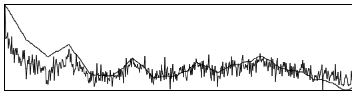
\includegraphics[clip,width=1.1\hsize]{img/POF.png}
  \caption{POF}\label{fig:POF}
\end{figure}

$$
\begin{aligned}
\mathrm{POF}[x_a, x_b]
&= \mathcal{F}^{-1}\left[\frac{\mathcal{F}\left[x_a(t)\right]^*}{|\mathcal{F}\left[x_a(t)\right]|}\mathcal{F}\left[x_b(t)\right]\right] \\
&= \mathcal{F}^{-1}\left[\frac{X_a^*(\omega)}{|X_a(\omega)|}X_b(\omega)\right]
\end{aligned}
$$


直接スペクトル拡散方式(図\ref{fig:DS})による測距システムの変復調方式を図\ref{fig:DME2}に示す.

\begin{figure}[p]\centering
  \hspace{-2mm}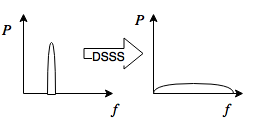
\includegraphics[clip,width=1.1\hsize]{img/DS.png}
  \caption{DS}\label{fig:DS}
\end{figure}

\begin{figure}[p]\centering
  \hspace{-2mm}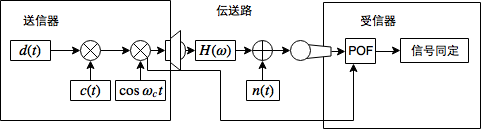
\includegraphics[clip,width=1.1\hsize]{img/DME2.png}
  \caption{DME2}\label{fig:DME2}
\end{figure}

\begin{figure}[p]\centering
  \hspace{-2mm}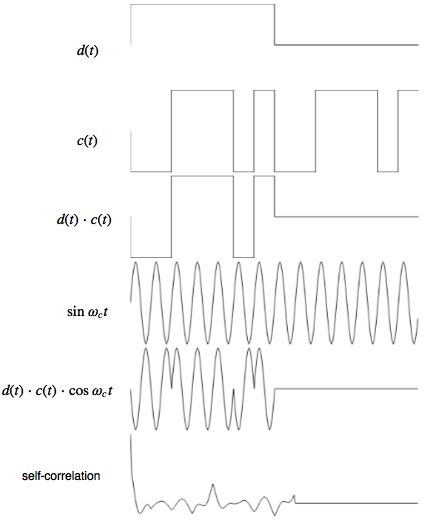
\includegraphics[clip,width=1.1\hsize]{img/DSSS.png}
  \caption{DSSS}\label{fig:DSSS}
\end{figure}

搬送波には1000Hzサイン波を,拡散符号にはM系列を用い,変調にはバイナリ位相シフトキーイング(BPSK)を使った.

復調した受信信号が雑音か有効な信号かを決定する処理を信号同定という.
伝送路における伝達関数 $H(\omega)$ において室内残響の影響
としてマルチパスによるを受けてしまう(図\ref{fig:multipath}).

\begin{figure}[pb]\centering
  \hspace{-2mm}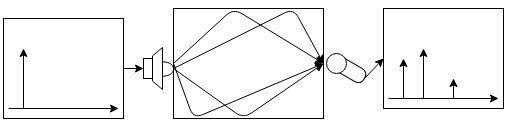
\includegraphics[clip,width=1.1\hsize]{img/multipath.png}
  \caption{multipath}\label{fig:multipath}
\end{figure}


そこで,同期パルスを測距用信号と,伝搬路を測定する参照波としてのサウンダ(sounder)信号の二つに分離した.
同期パルスから $n$ 秒後にサウンダ信号を送り,
その二つの信号の相関を取ることで,
背景雑音とは別にパルス位置を特定することが可能になる(図\ref{fig:sounder}).

\begin{figure}[pb]\centering
  \hspace{-2mm}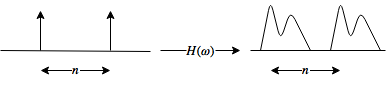
\includegraphics[clip,width=1.1\hsize]{img/sounder.png}
  \caption{sounder}\label{fig:sounder}
\end{figure}

さらにサウンダ信号と測距信号は互いに異なる同周期のM系列を用いた.
サウンダ信号と測距信号を判別しやすくするためである.

この時刻が $n$ 秒ずれた二つの信号に対して時間窓で区切って相互相関をとることで,
信号が最も相関している区間,つまり信号の位置を特定することができる.
最後に,その区間相関値を閾値処理することで信号の到来を決定する.
今回は最大相関値前方での40\%の相関値を超えたピークを到来時刻としている.

相関関数の計算にはウィーナー=ヒンチンの定理を使い周波数領域での複素乗算としてFFTを使って計算することで計算量を減らすことができる.
長さの異なる信号の高速フーリエ変換には重畳加算法\cite{overwrap}を使った.


\begin{figure}[p]
  \centering
  \includegraphics[clip,width=1.05\hsize]{img/026.jpeg}
  \caption{変復調回路}\label{fig:henpuku}
\end{figure}


\begin{figure}[p]
  \centering
  \includegraphics[clip,width=1.05\hsize]{img/029.jpeg}
  \caption{信号同定過程}\label{fig:shousai}
\end{figure}




\clearpage

\subsection{Barker coded chirpを用いたパルス圧縮}

これまでに測距・同期パルス(信号)の送受信による同期と測距および相対位置推定の手法について述べた.
ここでは,測距・同期精度を高くするための,信号検出手法について述べる.

信号検出においてSN比を最大化するフィルタを整合フィルタと呼び(図\ref{fig:matched_filter}),それは元信号との自己相関に等しい\cite{seigoufilter}.
理想的には整合フィルタを通した結果がデュラックのデルタ関数に近いことが望ましい.
しかしながら,そのような信号は短時間に大電力のパルスとなるため,送信機器の送信電力や回路の容量に物理的な制約があるため,そのような信号の送信は不可能である.
そこで,パルス圧縮と呼ばれる手法が使われている\cite{pulsecompress}.
パルス圧縮は,送信パルスを時間周波数方向へエネルギーを拡散させ,受信時にフィルタと高SN比で鋭いピークをもつようにする手法である.

音声パルスで同期する場合,音声信号のサンプリング周波数44100[Hz]と仮定すると,1サンプルあたりの時間解像度は約22.6$\mu$s,距離解像度は7.7mm(音速340[m/s]を仮定)となる.
人間の聴覚特性として$\pm$1msの誤差で別音源として聴こえることが知られている.
戦術の先行音効果により,必要な同期精度を$\pm$1msとすると,同期はおよそ$\pm$5サンプル以内の誤差に留める必要がある.
このような高精度のパルス検出のため,提案手法では複数のパルス圧縮方式を組み合わせる.

ここで,本手法に適用したパルス信号であるChirp信号について述べる.波形を図\ref{fig:chirpsig}に示し,スぺクトログラムを図\ref{fig:chirpsig2}に示す.
Chirp信号は,方形パルスを周波数方向へ掃引することで,図\ref{fig:chirppulse_amb}に示すように,通常パルスと同じ電力で時間方向の精度をより向上させることができることで知られている.
Barker符号(図\ref{fig:barkercode})はパルス圧縮の一種で,同期点以外での自己相関関数の絶対値の最大が$1/N$となる長さ$N$の有限長系列で,長さ13まで存在し,相関特性が長さ13の場合,ピークが13倍,レンジサイドローブが1/13倍となるような,ディラックの$\delta$関数に近い理想的な相関特性を持つことで知られている.

さらに,先行研究\cite{shibata13}のパルス圧縮に比べ,より強力なパルス圧縮として,
より狭い時間範囲にエネルギーを集中させることで,
上記の二つのパルス圧縮技術を組み合わせて,Chirp信号をBarker符号を用いてBPSKで変調した.
BPSKは位相0を0,位相$\pi$を1とする位相偏移変調で,位相変化を2値とする.
図\ref{fig:chirpqi}にBPSKの信号空間ダイアグラムを示す.

他にも,スマートデバイスのマイクロホンの周波数受信特性はそのハードウェアによって異なっている.
このため,BPSKの搬送波に特定の周波数を用いるのはハードウェアによっては最適ではない可能性がある.
これに対して,BPSKの搬送波に全帯域に対して掃引するChirp信号を用いる.
これにより,スマートデバイスのマイクロホンの周波数受信特性による差異を抑えることができると期待される.

\begin{figure}[pb]\centering
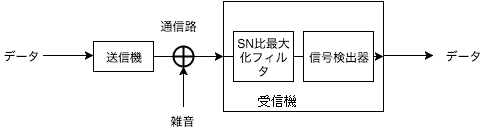
\includegraphics[clip,width=1.05\hsize]{img/matched_filter.png}
\caption{送受信モデルと整合フィルタ}\label{fig:matched_filter}

\end{figure}



\begin{figure}[pb]\centering
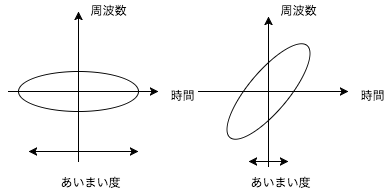
\includegraphics[clip,width=0.9\hsize]{img/aimai.png}\\
通常パルス~ ~ ~ ~ ~ ~ ~ ~ ~ ~ ~ Chirpパルス
\caption{Chirpパルスによるピーク曖昧度}\label{fig:chirppulse_amb}

\end{figure}

\begin{figure}[pb]\centering
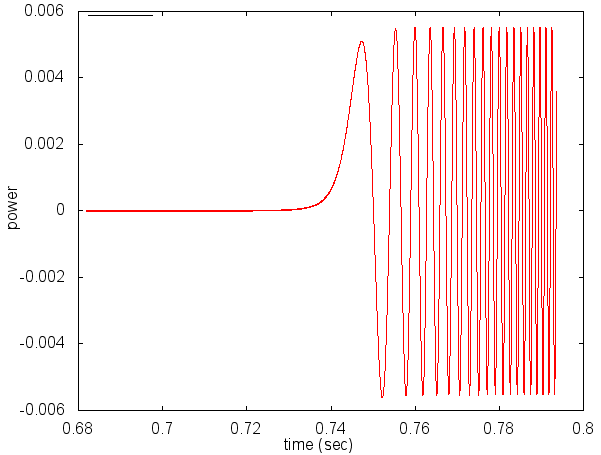
\includegraphics[clip,width=1.0\hsize]{img/chirp.png}
\caption{本手法で用いたChirp信号波形}\label{fig:chirpsig}

\end{figure}

\begin{figure}[pb]\centering

\includegraphics[clip,width=0.7\hsize]{img/chirp_spectogram.png}\\
\caption{本手法で用いたChirp信号スぺクトログラム}\label{fig:chirpsig2}

\end{figure}


\begin{figure}[pb]\centering
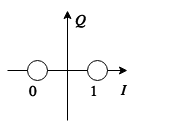
\includegraphics[clip,width=0.27\hsize]{img/chirp_qi.png}
\caption{BPSK信号空間ダイヤグラム}\label{fig:chirpqi}
\end{figure}




\begin{figure}[pb]\centering
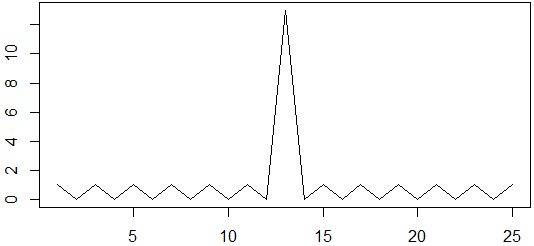
\includegraphics[clip,width=0.9\hsize]{img/barkercode.png}
\caption{Barker符号(13列)の自己相関形}\label{fig:barkercode}
\end{figure}

\begin{figure}[pb]\centering
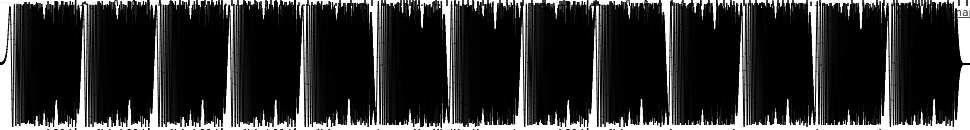
\includegraphics[clip,width=1.0\hsize]{img/barker_chirp.png}
\caption{13列Barker符号のBPSK変調信号(Chirp信号搬送波)}\label{fig:barker_chirp}
\end{figure}

\begin{figure}[pb]\centering
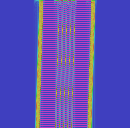
\includegraphics[clip,width=0.75\hsize]{img/barker_coded_chirp.png}
\caption{13列Barker符号のBPSK変調信号(Chirp信号搬送波)のスペクトルグラム(シミュレーション)}\label{fig:barker_coded_chirp}
\end{figure}


\begin{figure}[pb]\centering
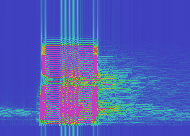
\includegraphics[clip,width=0.75\hsize]{img/barker_coded_chirp_err.png}
\caption{13列Barker符号のBPSK変調信号(Chirp信号搬送波)のスペクトルグラム
(MacBookAirによる実環境での自身の信号の計測結果)}\label{fig:barker_coded_chirp_err}
\end{figure}


\begin{figure*}[pb]\centering
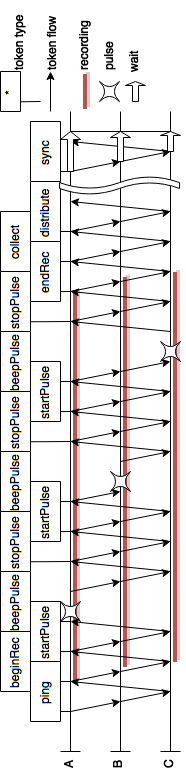
\includegraphics[clip,width=0.85\hsize]{img/flowchart.png}
\caption{システム動作のダイアグラム}\label{fig:pulsediagram}
\end{figure*}

\begin{figure}[pb]\centering
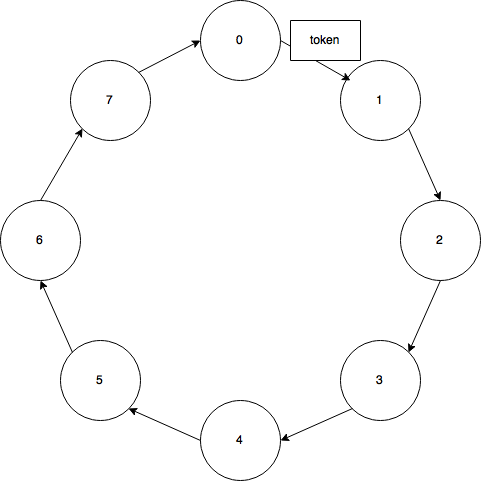
\includegraphics[clip,width=0.85\hsize]{img/chord_ring_network.png}
\caption{ネットワーク上でのトークンパッシング}\label{fig:scheduling}
\end{figure}


\begin{figure}[pb]\centering
\vspace{2mm}
\begin{small}
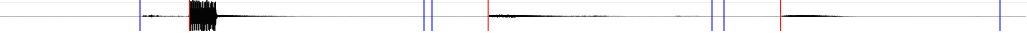
\includegraphics[clip,width=1.0\hsize]{img/rawdata.png}\\
A端末自身のパルス~ ~ ~ ~
B端末のパルス~ ~ ~ ~ ~
C端末のパルス\\\vspace{0.5mm}

\includegraphics[clip,width=0.8\hsize]{img/spectrogram.png}\hspace{1cm}\\
A端末自身のパルス~ ~ ~ ~ ~ ~ ~ ~ ~
B端末のパルス\\\vspace{0.5mm}
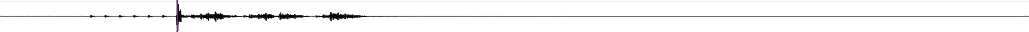
\includegraphics[clip,width=1.0\hsize]{img/corrA.png}\\
A端末のパルスに整合フィルタをかけたもの\\\vspace{0.5mm}
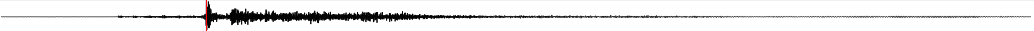
\includegraphics[clip,width=1.0\hsize]{img/corrB.png}\\
B端末のパルスに整合フィルタをかけたもの\\\vspace{0.5mm}
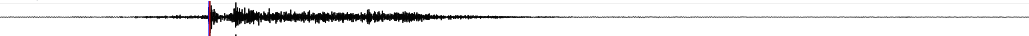
\includegraphics[clip,width=1.0\hsize]{img/corrC.png}\\
C端末のパルスに整合フィルタをかけたもの\\
\vspace{1mm}
\caption{A端末で観測したABC端末のパルス信号}\label{fig:corr}

\end{small}
\vspace{1mm}
\end{figure}


\section{システムクロック校正}

端末のシステムクロックの進みかたはハードウェアごとに微妙に異なる.
そのため,同期してから長時間経つと,次第に端末間で遅延が生じる.
このことは,同一音源を同期的に再生し続けると,次第にずれが聞き取れるようになってくることを意味する.
この遅延を検出する手法について述べる.

端末 A のクロックを $S_A$,
端末 B のクロックを $S_B$ して,
時刻 $t$ 後に
A のサンプル数が $i$ ,
B のサンプル数が $i+d$ だけ異なっているとする(図\ref{fig:phaseshift2}).
このとき,Aを基準とした遅延比率 $S_B/S_A$ を求めたい.

\begin{figure}[p]\centering
  \hspace{-2mm}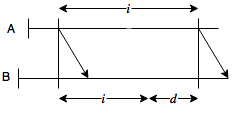
\includegraphics[clip,width=1.1\hsize]{img/phase_shift2.png}
  \caption{phaseshift2}\label{fig:phaseshift2}
\end{figure}

図より

$$\begin{aligned}
\frac{i}{S_A} &= \frac{i+d}{S_B} = t \\
\frac{S_B}{S_A} &= \frac{i+d}{i}
\end{aligned}$$

である.
遅延の検出においては,端末間の相対距離に変化がない限り,
端末Aが端末Bへとパルスを発生するだけで良く,
端末BはAへと返答パルスを返す必要はない.
既に同期済みでありAからBへの伝搬時間は算出済みだからである.



\section{音圧校正}
スマートデバイス毎にマイクロホンやスピーカのアンプ出力は異なるため,そのままではDBAP法は使えない.
ここでは,機器ごとの音圧を校正する手法を示す.

LTI(線形時不変)システムを仮定する.
$N$ 台の端末の番号を $i,j \in \{1\dots N\}$ とする.
端末 $i$ から端末 $j$ への信号伝達を考える.
$e$ を端末 $i$ で生成した単位振幅,
$v_i$ を端末 $i$ のスピーカアンプの増幅係数,
$m_j$ を端末 $j$ のマイクロホンアンプの増幅係数,
$d_{ij}=d_{ij}$ を $ij$ 間の測定距離,
$x_{ij}$ を $j$ が観測した $i$ からの信号の振幅とする.
音波の振幅は距離に反比例して減衰することが知られているので,
音声信号の伝達は

\begin{figure}[p]\centering
  \hspace{-2mm}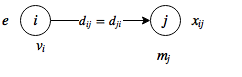
\includegraphics[clip,width=1.1\hsize]{img/sound_pressure_calibration.png}
  \caption{soundpressurecalibration}\label{fig:soundpressurecalibration}
\end{figure}

$$
e v_i \frac{1}{d_{ij}} m_j = x_{ij}
$$

とモデル化できる(図\ref{fig:soundpressurecalibration}).
このとき,ある端末 $k$ の出力係数 $v_k$ と他の端末 $i$ の出力係数 $v_i$ との比 $v_i/v_k$ を求めたい.

$$
e v_i m_j = x_{ij}d_{ij}
$$

なので

$$\begin{aligned}
\frac{e v_j m_j}{e v_k m_j} &= \frac{x_{ij} d_{ij}}{x_{kj} d_{kj}} \\
\frac{v_j}{v_k} &= \frac{x_{ij} d_{ij}}{x_{kj}d_{kj}} \\
\end{aligned}$$

である.
観測した振幅 $x_{ij}$ および測定距離 $d_{ij}$ は誤差を含むので,
それらを平均した $\hat{v_i}$ は

$$
\frac{\hat{v_i}}{v_k} = \frac{1}{N} \sum_{i\neq j \neq k} \frac{x_{ij} d_{kj}}{x_{kj}d_{ij}} \\
$$

と定義できる.$d_{ii}$ のときは距離が0となりゼロ除算が発生するので,
$i\neq j \neq k$ としている.

一番出力の低い端末 $k$ の出力係数 $v_k$ を基準とすることで,
すべての端末において定格出力を守ることができる.

\section{隣接ノードでない端末間の同期,音圧校正,クロック校正}


互いに互いの信号を検出できなかったノード間での校正を考える.
図\ref{fig:networktopology}に隣接ノードではない端末を含むネットワークを示す.

\begin{figure}[p]\centering
  \hspace{-2mm}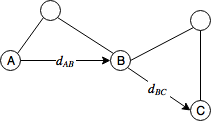
\includegraphics[clip,width=1.1\hsize]{img/network_topology.png}
  \caption{networktopology}\label{fig:networktopology}
\end{figure}

このとき端末 A と端末 C 間では同期・測距ができていないが,
互いに端末 B とは同期・測距できているという状況である.

\subsection{同期}

時刻の基準となる
端末 $A$ がパルスを発した時間を $t_{AA}$ として
そのパルスが端末 $B$ に届いた時間は $t_{AB}$ とする.
また,
端末 $B$ がパルスを発した時間を $t_{AB}$ として
そのパルスが端末 $C$ に届いた時間は $t_{BC}$ とする.
そしてそれぞれの伝達時間を $d$ とすると図\ref{fig:reldelay}のようになる.

\begin{figure}[p]\centering
  \hspace{-2mm}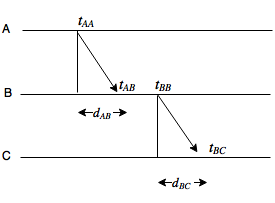
\includegraphics[clip,width=1.1\hsize]{img/rel_delay.png}
  \caption{reldelay}\label{fig:reldelay}
\end{figure}

このとき,まず端末 $C$ は端末 $B$ と同期して,
その後端末 $B$ と端末 $A$ の時刻ずれ情報をもとにさらに端末 $A$ との同期ができる.


\subsection{音圧校正}

端末 $A$ を基準に音圧校正を考えると

$$
\frac{v_B}{v_A} = \frac{x_{iB} d_{iB}}{x_{AB}d_{AB}} \\
\frac{v_C}{v_B} = \frac{x_{iC} d_{iC}}{x_{BC}d_{BC}} \\
$$

であるので

$$
\frac{v_C}{v_A} =
\frac{v_B v_C}{v_A v_B} =
\frac{x_{iB} x_{iC} d_{iB} d_{iC}}{x_{AB} x_{BC} d_{AB} d_{BC}}
$$

とすれば端末 A と端末 C の出力比率を求められる.

\subsection{クロック校正}


\section{同期・測距・校正手法のための制御システム}
同期のためには複数の端末がパルスを出し合わなければならないが,
いつどの端末がパルスを出すのか,といったスケジューリングをどうするかについて述べる(図\ref{fig:TDMA}).

\begin{figure}[p]\centering
  \hspace{-2mm}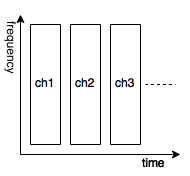
\includegraphics[clip,width=1.1\hsize]{img/TDMA.png}
  \caption{TDMA}\label{fig:TDMA}
\end{figure}

図\ref{fig:network2}にシステム全体のネットワーク構成を示す.

\begin{figure}[p]\centering
  \hspace{-2mm}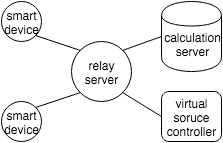
\includegraphics[clip,width=1.1\hsize]{img/network2.png}
  \caption{ネットワーク構成}\label{fig:network2}
\end{figure}

基本的には端末間の通信を中継するリレーサーバを中心としたスター型ネットワークである.
また,スピーカアレイに参加しない特別なノードとして,
計算用ノードと仮想音源を設定する制御用ノードがある.


今回の実装では中継サーバが同期アルゴリズムを制御している.
すべてのコマンドはリクエスト-レスポンスで成り立っており,リクエストを受けた端末は必ずレスポンスを返さねばならない.
まず,中継サーバはスピーカアレイを構成する端末に対して ping コマンドを送信し,
アレイに参加できる端末を確認する.
次に,全端末に対して録音をするように beginRec コマンドを送信する.
そして,各端末の放つパルスが排他的になるように,
パルスを放つ端末ごとにstartPulse,beepPulse,stopPulseコマンドを繰り返し送信する.
startPulseとstopPulseコマンドは,
この時間区間内にいずれかの端末からパルスが発信されることを示すもので,
後にパルス位置を検出するときの計算量を減らすためのコマンドである.
beepPulseは任意の一台の端末に対して,パルスを送信するように促すコマンドである.
すべての端末が互いに排他的にパルス発生し終えると,
最後にstopRecという録音終了コマンドを送信する.
その後,collectコマンドで各端末が録音したデータを集計し,
計算用サーバへ送信する(図\ref{fig:pulsediagram}).
計算用サーバは,それぞれの端末間のパルスの受信時刻を
先述の手法で検出し,相対信号伝達時間と相対距離計測,空間配置推定する.
その後,それらの情報を中継サーバを介して制御用端末へ送信する.




\begin{figure*}[p]\centering
\hspace{-2mm}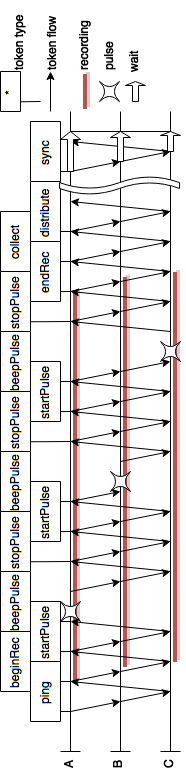
\includegraphics[clip,height=1.5\hsize]{img/flowchart.png}
\caption{システム動作のダイアグラム}\label{fig:pulsediagram}
\end{figure*}


\section{仮想音源配置によるDBAPアレイスピーカ制御システム}

仮想音源を配置し制御するための端末のユーザインターフェースを示す(図\ref{fig:relpos}).

\begin{figure}[p]\centering
  \hspace{-2mm}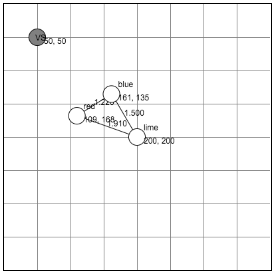
\includegraphics[clip,width=1.1\hsize]{img/relpos.png}
  \caption{仮想音源配置ユーザインタフェース}\label{fig:relpos}
\end{figure}

図のように推定した端末の分布図と,仮想音源を表示する.
仮想音源VSをドラッグすることで,DBAP法によって出力する振幅を計算し,各端末へ振幅を配信することで音像定位する.
また,音を鳴らしながら音源を移動させることも可能である.

